\begin{center}
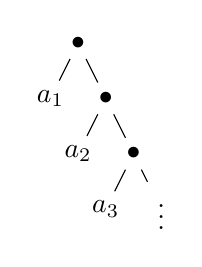
\begin{tikzpicture}[sibling distance=2em, level distance=2em]
  \node {\(\bullet\)}
    child { node {\(a_1\)} }
    child { node {\(\bullet\)}
      child { node {\(a_2\)}}
      child { node {\(\bullet\)}
        child { node {\(a_3\)}}
        child { node {\(\vdots\)}
    }}};
\end{tikzpicture}
\qquad
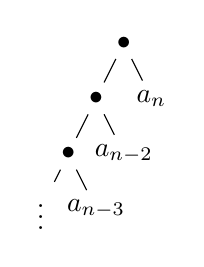
\begin{tikzpicture}[sibling distance=2em, level distance=2em]
  \node {\(\bullet\)}
    child { node {\(\bullet\)}
      child { node {\(\bullet\)}
        child {node {\(\vdots\)}}
        child {node {\(a_{n-3}\)}}}
      child { node {\(a_{n-2}\)}}
        }
    child { node {\(a_n\)} };
\end{tikzpicture}
\qquad
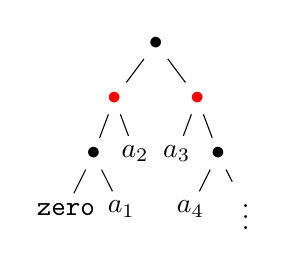
\begin{tikzpicture}[level distance=2em, level 3/.style={sibling distance=2em}, level 2/.style={sibling distance=1.5em}, level 1/.style={sibling distance=3em}]
  \node {\(\bullet\)}
  child { node[color=red] {\(\bullet\)}
    child { node {\(\bullet\)}
      child {node {\texttt{zero}}}
      child {node {\(a_1\)}}}
    child { node {\(a_2\)}}
  }
  child { node[color=red] {\(\bullet\)}
    child { node {\(a_3\)} }
    child { node {\(\bullet\)}
      child { node {\(a_4\)}}
      child { node {\(\vdots\)}
      }}};
\end{tikzpicture}
\end{center}